\chapter{Implementace}
\label{chap:implementace}
V kapitole~\ref{chap:analysis} byla analyzována hra Berušky 2, která se stala vzorem pro hru implementovanou v rámci této práce. Způsob, jakým je hra implementována, je uveden na diagramu~\ref{fig:gameDiagram}. V následující podkapitolách budou popsány jeho jednotlivé části a tím i objasněna herní architektura.

TODO...jak byla testovana funkcnost

\begin{figure}[htb]
\centering
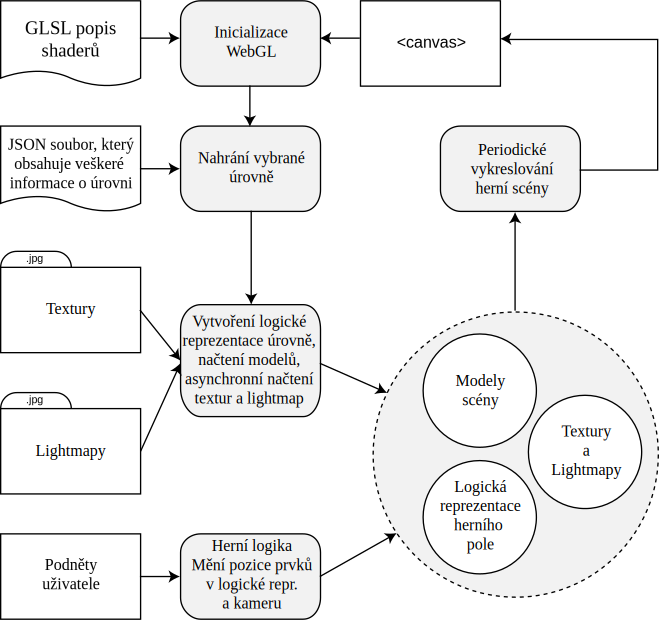
\includegraphics[width=0.8\textwidth]{gameDiagram}
\caption{Architektura hry Berušky 2 WebGL}
\label{fig:gameDiagram}
\end{figure}

\section{Inicializace}
Inicializace elementu \texttt{<canvas>} je prvním krokem, který je potřeba vykonat. Tím, že získáme referenci na jeho \texttt{webgl} kontext, můžeme přejít k dalšímu kroku, který nastaví vertex a fragment shadery. Popis funkčnosti shaderů je proveden pomocí jazyka GLSL, jehož ukázky byly uvedeny u popisu grafické pipeline (\ref{subsection:pipeline}). Zdrojové kódy jsou obsaženy v HTML dokumentu uvnitř těchto elemtentů:
\begin{itemize}
\item Vertex Shader \\ \texttt{\textless script id="per-fragment-lighting-vs"\ type="x-shader/x-vertex"\textgreater}
\item Fragment Shader \\ \texttt{\textless script id="per-fragment-lighting-fs"\ type="x-shader/x-fragment"\textgreater}
\end{itemize}

V implementaci je hra inicializována pomocí funkce \texttt{webGLStart()}, která mimo jiné nastavuje způsob zpracování událostí vytvářených uživatelem.

\section{Nahrání vybrané úrovně}
Po inicializaci je přistoupeno k nahrání úrovně vybrané hráčem. Každá z úrovní je představována samostatným JSON souborem, který je asynchronně nahrán (\ref{subsection:AJAX}) ze serveru.

\subsection*{JSON soubor}
\label{subsection:navrhJSON}
Tento soubor obsahuje kompletní informace, které jsou potřebné pro zobrazení dané herní úrovně. Jedná se tak o hlavní součást celé hry, bez které by nemohla fungovat. Soubor vzniká exportem potřebných informací z původní hry a jeho hlavní součásti jsou popsány v následujících odstavcích.

\myparagraph{Informace o materiálech}
Materiály jsou použity k otexturování modelů. Rozdíl mezi materiálem a texturou je takový, že materiál se obecně může skládat z více textur, které se pak vzájemně prolínají. Lze tak mít například materiál, který vznikne složením z textur zdi a mechu. Výhoda je v tom, že složitější textury lze složit z jednodušších a není tedy potřeba uchovávat nadbytečná data. Každý z materiálů má v souboru jména textur, ze kterých se skládá, a také své unikátní jméno, pomocí něhož se následně objekty scény na tento materiál odkazují. Ukázka popisu materiálu je uvedena ve zdrojovém kódu~\ref{code:jsonMaterial}.

\begin{lstlisting}[caption=Objekt \texttt{material} vstupního souboru JSON,label=code:jsonMaterial]
{
  "type" : "material",
  "name" : "256_p-d1-256",
  "transparent" : "0",
  "z_buffer_mask" : "1",
  "z_buffer_test" : "1",
  "backface_culling" : "1",
  "diffuse_color" : "1",
  "specular_color" : "0",
  "textures" : [ "s1_0013.jpg" ]
}
\end{lstlisting}

\myparagraph{Obálky objektů herní scény}
Málokterý ze složitějších objektů je složen pouze z jednoho modelu. Ve chvíli, kdy celkový model objektu rozdělíme na části, je možné tyto části samostatně transformovat či měnit materiál, který používají. Avšak v okamžik, kdy chceme nějakým způsobem transformovat celý objekt, je vhodné mít všechny modely objektu v jakési obálce. Tato obálka má v souboru své identifikační číslo, které slouží k identifikaci všech jejích modelů. Identifikační číslo je potřebné pouze tehdy, pokud potřebujeme s obálkou transformace provádět a je tedy využito pouze u dynamických objektů herní plochy.

\mysubparagraph{Modely}
Modely jsou v souboru reprezentovány strukturami, které obsahují informace o poloze modelů v rámci scény, o jejich barvě či například o materiálech, které jsou jim přiřazeny. Některé z modelů mají také další textury s předpočítanými stíny pro realističtější zobrazení scény - lightmapy. 

Ve zdrojovém kódu~\ref{code:jsonContainer} je uveden zjednodušený popis obálky, která obsahuje 1 model. Identifikační číslo \texttt{2} znamená, že se jedná o dynamický prvek scény (pokud by se jednalo o statický prvek, pak by číslo bylo \texttt{-1}). Pomocí položky \texttt{material} se model v tomto případě odkazuje na materiál, který byl popsán ve zdrojovém kódu~\ref{code:jsonMaterial}. Trojice prvků v poli \texttt{vertexPositions} vždy udává pozici vertexu ve scéně. O tom, které vertexy náleží geometrickým primitivám, ze kterých je model složen, rozhoduje pole \texttt{indices}. Zbylé položky pak obsahují informace potřebné pro správné namapování materiálů a lightmap.

\begin{lstlisting}[caption=Objekt \texttt{geometry\_container} vstupního souboru JSON,label=code:jsonContainer]
{
  "type" : "geometry_container",
  "name" : "exit.b2m",
  "container_id" : "2",
  "poly_id" : "17",
  "prvek" : "1",
  "geometry_objects" : [
   {
    "name" : "exit.b2m",
    "material" : "256_p-d1-256",
    "vertexPositions" : [-27.586000,2.008000,-34.421001,-27.586000,0.008000,-36.421001,
         47.704437,85.772964,6.669896,130.704437,85.772964,-3.330104],
    "vertexNormals" : [-1.000000,0.000000,0.000000,-1.000000,0.000000,0.000000],
    "vertexTextureCoords0" : [1.000000,1.000000,0.000000,0.000000,1.000000,0.000000],
    "vertexTextureCoords1" : [1.000000,1.000000,0.000000,0.000000,1.000000,0.000000],
    "vertexTextureCoordsLight" : [0.140625,0.328125,0.171875,0.328125,0.156250,0.359375],
    "indices" : [0,1,2,3,0,5]
   }
  ]
}
\end{lstlisting}

\myparagraph{Logická reprezentace herního pole}
Obálky modelů neobsahují žádnou informaci o tom, jaký typ objektu ve scéně představují. Z tohoto důvodu je nutné rozlišit to, co je vykreslováno na obrazovku, a s čím pracuje logika hry. Jak již bylo uvedeno v kapitole~\ref{chap:analysis}, herní pole je krychlové či kvádrové a je složeno z jednotlivých pozic, na kterých se mohou nacházet herní prvky. Je to právě logická reprezentace herního pole, která obsahuje informace o tom, který prvek se na které pozici nachází. Každý prvek logické reprezentace herního pole má opět své identifikační číslo, pomocí kterého se odkazuje na obálku modelu, který určuje jeho vzhled.  

Ve zdrojovém kódu~\ref{code:jsonLogic} je uveden popis herního pole o velikosti $6\times6$ a výšce $8$. Položka \texttt{level\_start} udává pozici, na kterou mají být přesunuty dynamické objekty, které jsou normálně umístěny v počátku souřadného systému scény. Herní pole zde obsahuje pouze jeden prvek, jehož typ je určen položkami \texttt{class} a \texttt{subclass} (identifikátory všech prvků jsou uvedeny v tabulce~\ref{table:itemClass}). Logický prvek se v tomto příkladu pomocí \texttt{container\_id} odkazuje na model, který byl popsán ve zdrojovém kódu~\ref{code:jsonContainer}. 

\label{code:jsonLogic}
\begin{lstlisting}
{
  "type" : "level_logic",
  "logic_level_size" : [ 6, 8, 6],
  "level_start" : [ 21.586000, -1.992000, -46.421001],
  "item_size" : "2",
  "level_items_num" : "1",
  "level_items" : [{
    "name" : "Exit - teleport - 1",
    "guid" : "4000",
    "class" : "4",
    "subclass" : "-1",
    "position" : [ 0, 5, 1 ],
    "rotation" : "0",
    "container_id" : "2"
  }]
}
\end{lstlisting}

\begin{table}
\label{table:itemClass}
\begin{center}
\begin{tabular}{ | l | l | l |}
\hline
\textbf{Prvek} & \textbf{itemClass} & \textbf{itemSubclass} \\ \hline
Beruška & 1 & 0 \\ \hline
Zeď & 2 & 0 \\ \hline
Východ & 4 & 0 \\ \hline
Bedna & 5 & 0 \\ \hline
Těžká bedna & 5 & 0 \\ \hline
Lehká bedna & 5 & 1 \\ \hline
Výbušnina & 6 & 0 \\ \hline
Kámen & 7 & 0 \\ \hline
Voda & 12 & 0 \\ \hline
Šnorchl & 13 & 0 \\ \hline
Hormonální vitamín & 13 & 5 \\ \hline
Závaží & 13 & 7 \\ \hline
Krompáč & 13 & 8 \\ \hline
Bortící se podlaha & 15 & 0 \\ \hline
Šikmina & 19 & 0 \\ \hline
\end{tabular}
\end{center}
\caption{Třídy a podtřídy prvků herního pole}
\end{table}

Jak si mohl pozorny čtenář všimnout, čísla, která označují typ prvku, nejdou sekvenčně za sebou. Je to způsobeno tím, že původní návrh hry Berušky 2 (desktopové verze) obsahoval více typů herních prvků, než jich bylo nakonec implementováno. 

\section{Vytvoření vnitřní reprezentace herní úrovně}
Každé struktuře vyskytující se v JSON souboru (popsáno v~\ref{subsection:navrhJSON}) přísluší odpovídající objekty a po jeho asynchronním načtení je soubor zpracován pomocí funkce \texttt{handleLoadedJSON}. Ta tento soubor sekvenčně prochází, rozpoznává jeho jednotlivé struktury a následně pomocí JavaScriptových konstruktorů vytváří odpovídající objekty, se kterými hra pracuje. V následujících odstavcích je uveden přehled těchto konstruktorů s jejich stručným popisem.

\myparagraph{\texttt{Material}}
Při vytváření objektu tímto konstruktorem jsou ze serveru asynchronně (\ref{subsection:AJAX}) nahrány textury, které materiál využívá. Z těch jsou následně vytvořeny texturovací buffery, které jsou nahrány do grafické paměti. Tím, že jsou do této paměti umístěny, je pak dosaženo rychlejšího vykreslování celé herní scény. Buffery jsou nastaveny tak, že pokud je textura oproti své původní velikosti zvětšována (upscaling), pak se použije lineární filtr, který na základě okolních pixelů dopočítá lineární interpolací barvu pixelu mezi nimi. Pro textury, které jsou naopak zmenšovány je vygenerována mipmapa, ze které se pak vybírá nejvhodnější verze textury. Všechny materiály jsou uchovávány v asociativním poli \texttt{materials}, kde jednotlivé klíče tohoto pole jsou samotné názvy materiálů. 

Ve zdrojovém kódu~\ref{code:loadingMaterial} je uveden příklad nahrání texturovacího bufferu vzniklého načtením první textury materiálu uvedeného ve zdrojovém kódu~\ref{code:jsonMaterial} do grafické paměti.

\begin{lstlisting}[caption=Příklad nahrání textury do grafické paměti,label=code:loadingMaterial]
// ...	
// Textura je zrcadlově obrácena kolem osy Y
// WebGL používá jiný souřadný systém
gl.pixelStorei(gl.UNPACK_FLIP_Y_WEBGL, true);
// Nastavení aktuálně zpracovávaného bufferu textury
gl.bindTexture(gl.TEXTURE_2D, materials["256_p-d1-256"].buffers[0]); 
// Nahrání textury do grafické paměti
gl.texImage2D(gl.TEXTURE_2D, 0, gl.RGBA, gl.RGBA, gl.UNSIGNED_BYTE, 
              that.textures[temp].image);
// Nastavení filtru, kterým bude textura zvětšována
gl.texParameteri(gl.TEXTURE_2D, gl.TEXTURE_MAG_FILTER, gl.LINEAR);
// Nastavení filtru, kterým bude textura zmenšována
gl.texParameteri(gl.TEXTURE_2D, gl.TEXTURE_MIN_FILTER, 
                 gl.LINEAR_MIPMAP_NEAREST);
// Vygenerování mipmapy
gl.generateMipmap(gl.TEXTURE_2D);
// ...
\end{lstlisting}

\myparagraph{\texttt{Lightmap}}
Objekt vytvořený tímto konstruktorem je až na pár detailů stejný jako objekt konstruktoru \texttt{Material}. Lightmapy jsou taktéž načítány asynchronně a ukládány do paměti grafické karty, avšak vzhledem k tomu, že se z původní hry nepodařilo všechny lightmapy vyexportovat, je jejich použití vypnuto.

\myparagraph{\texttt{GeometryContainer}}
\label{paragraph:obálky}
Tento konstruktor vytváří obálku jednotlivých modelů herní scény. Podle toho, zda obálka obsahuje identifikační číslo, rozlišujeme mezi obálkami dynamických a statických objektů scény a umísťujeme je do odpovídajících polí. Pro dynamické obálky je to asociativní pole \texttt{dynamicItems}, jehož klíči jsou identifikátory obálek a pro statické obálky je to pole staticItems, kde jsou obálky seřazeny tak, jak byli načítány ze vstupního souboru. Každá z obálek ve svém poli \texttt{objects} uchovává modely, které jí náleží. 

\myparagraph{\texttt{GeometryObject}} 
Objekt vytvořený tímto konstruktorem obsahuje veškeré informace spojené s vykreslováním modelu. Důležité je to, že jsou zde uloženy buffery, do kterých jsou nahrány informace o pozicích vertexů, směrech jejich normál a dále pak například o souřadnicích potřebných pro správné namapování materiálu. Ve zdrojovém kódu~\ref{code:vertexBuffer} je uveden příklad nahrání pozic vertexů ze struktury, která v JSON souboru reprezentuje načítaný model.

\begin{lstlisting}[caption=Příklad nahrání pozic vertexů do bufferu,label=code:vertexBuffer]
// Vytvoření vertex position bufferu
this.vertexPositionBuffer = gl.createBuffer();
gl.bindBuffer(gl.ARRAY_BUFFER, this.vertexPositionBuffer);
// Načtení dat z JSON souboru
gl.bufferData(gl.ARRAY_BUFFER, new Float32Array(model.vertexPositions), 
              gl.STATIC_DRAW);
this.vertexPositionBuffer.itemSize = 3;
this.vertexPositionBuffer.numItems = model.vertexPositions.length / 3;
\end{lstlisting}

\myparagraph{\texttt{Logic}}
\label{paragraph:logic}
Objekt tohoto konstruktoru obsahuje veškeré informace spojené s herním polem a také veškerou herní logiku. Prvky herního pole jsou reprezentovány objekty konstruktoru \texttt{LogicItem}. Vzhledem ke svému rozsahu je tento objekt popsán samostatně v podkapitole~\ref{section:implementationLogic}.

\myparagraph{\texttt{LogicItem}}
Objekty představují jednotlivé herní prvky, které obsahují informace o jejich typu, pozici a aktuálním natočení. Každý z prvků má své unikátní identifikační číslo, které slouží k propojení s obálkou jeho modelu.

\section{Herní logika a podněty uživatele}
\label{section:navrhLogika}
V implementované hře je každý podnět uživatele zpracováván herní logikou, která je implementována na základě analýzy hry Berušky 2 provedené v kapitole~\ref{chap:analysis}. Pro vyhodnocení podnětu uživatele je volána funkce \texttt{gameStep()}. Ta představuje herní krok, ve kterém je vždy zjištěna pozice aktuálně zvolené berušky a dle jejího natočení se pak určí pozice, na kterou hodlá přejít. Podle toho, jaký typ prvku se na následující pozici nachází, jsou vykonávány akce, jejichž popis je uveden v následujícím přehledu.

\begin{itemize}
\item \textbf{Nic} - pokud je beruška v nejnižší úrovní herního pole, pak je krok proveden. Pokud ne, pak je nejdříve zkontrolován obsah pozice, která je pod místem, kam hodlá beruška přejít.
\begin{itemize}
\item Pod místem je \textit{šikmina}. Pokud je šikmina správně natočena, pak se ještě zkontroluje, zda nevede šikmina pod vodní hladinu, kde by beruška potřebovala šnorchl. Při splnění všech podmínek je krok následně proveden.
\item Pod místem je \textit{bortící se podlaha}. Ta se propadne pouze v případě, že má beruška ve svém inventáři závaží.
\item Pod beruškou je jiná \textit{beruška} - přechod se neprovede.
\item Pokud zde není \textit{žádná pevná plocha}, na které by beruška mohla stát (zeď, bedna, východ, výbušnina či kámen), pak se krok neprovede. 
\end{itemize}
\item \textbf{Beruška} - krok se neprovede, jinou beruškou nelze přímo pohnout.
\item \textbf{Zeď} - krok se neprovede, zeď je statickým prvkem herního pole.
\item \textbf{Východ} - beruška opouští herní pole. Pokud je to beruška poslední, pak končí hra.
\item \textbf{Bedna} - zjistí se celková váha všech posouvaných beden a pokud je nižší nebo rovna beruščině síle, pak se bedna/bedny v daném směru posouvají. Pokud pod sebou posunutá bedna nemá podklad, pak je její pozice upravena tak, aby ho pod sebou měla.
\item \textbf{Výbušnina} - zjistí se, co se nachází na pozici, kam by měla být výbušnina posunuta. Pokud je na následující pozici bedna, pak je výbušnina i bedna odstraněna a beruška zůstává na své původní pozici. Pokud za výbušninou není bedna, pak se stejně jako bedna posune.
\item \textbf{Kámen} - prohledá se inventář berušky a pokud obsahuje krompáč, pak je kámen odstraněn s tím, že beruška zůstává na své původní pozici. V opačném případě se krok neprovede.
\item \textbf{Šnorchl} - beruška může vlastnit pouze jeden. Pokud ho tedy ještě ve svém inventáři nemá, pak se šnorchl odstraní z herního pole, přidá se do beruščina inventáře a ta samotná je posunuta na pozici, kde se šnorchl nacházel.
\item \textbf{Hormonální vitamín} - situace je obdobná jako u šnorchlu.
\item \textbf{Závaží} - opět stejná situace jako u šnorchlu.
\item \textbf{Krompáč} - krompáč se odstraní a přidá se do inventáře pouze v případě, že v něm má beruška místo. Maximální počet krompáčů, který může mít beruška v jeden okamžik v inventáři je 4.
\item \textbf{Bortící se podlaha} - může se nacházet i před beruškou, avšak krok který by vedl k tomu, že by beruška byla pod podlahou se neprovede.
\item \textbf{Šikmina} - zde opět záleží na natočení šikminy. Vzhledem k tomu, že se nad šikminou může nacházet jakýkoliv jiný herní prvek, je krok při správném natočení šikminy rozdělen na 2 fáze. Nejprve je beruška pro potřeby výpočtu přesunuta nad šikminu a následně je krok prováděn z tohoto umístění. 
\end{itemize}

Je také důležité připomenout, že při každém posunu prvků je potřeba zkontrolovat, zda se posunem nedostaly do místa, kde by levitovaly ve vzduchu. Pozice se musí upravit s tím, že pokud se v nově vzniklém sloupci prvků nachází některé výbušné bedny, pak při úpravě vertikální polohy sloupce výbušné bedny odstraňují normální bedny, které mají pod sebou. Stejně tak je potřeba kontrolovat, zda se v nově vzniklém sloupci prvků nenachází bortící se podlaha. Pokud je váha nad bortící se podlahou vyšší jak 1, pak je bortící se podlaha odstraněna a sloupec objektů je vertikálně posunut.

\subsection*{Objekt herní logiky}
\label{section:implementationLogic}
Při vytvoření tohoto objektu jsou z JSON souboru načteny potřebné informace a podle nich jsou pak dopočítány ty zbylé. Prvky herního pole se stejně jako obálky modelů (\ref{paragraph:obálky}) dělí na statické a dynamické a jsou uloženy v odpovídající polích \texttt{staticItems} a \texttt{dynamicItems} tohoto objektu (neplést s poli určenými pro obálky modelů, které jsou uloženy v globálních polích se stejnými názvy). Statické prvky jsou indexovány pomocí čísla, které je odvozeno z pořadí při jejich načítání. Dynamické prvky jsou naopak indexovány svým identifikačním číslem. 

Jak již bylo uvedeno v~\ref{paragraph:logic}, tento objekt obsahuje veškerou herní logiku v podobě funkcí, které jsou rozděleny do několika kategorií. Kategorie a odpovídající komentované přehledy jsou uvedeny v tabulce~\ref{table:logicCategories}.

\begin{table}
\label{table:logicCategories}
\begin{center}
\begin{tabular}{ | l | l |}
\hline
\textbf{Kategorie} & \textbf{Zdrojový kód} \\ \hline
Práce s beruškami & \ref{code:logicBug} \\ \hline
Práce s inventářem & \ref{code:logicInventory}\\ \hline
Získávání reference na prvky & \ref{code:logicReference}\\ \hline
Výpočet váhy prvků & \ref{code:logicWeight} \\ \hline
Posun prvků & \ref{code:logicMove} \\ \hline
Odstraňování prvků & \ref{code:logicRemove} \\ \hline
Herní krok & \ref{code:logicGameStep}\\ \hline
\end{tabular}
\end{center}
\caption{Kategorie funkcí herní logiky}
\end{table}

\begin{lstlisting}[caption=Funkce pro práci s beruškami,label=code:logicBug]
/**
* Vybere berušku s daným ID.
* @param id ID berušky, která má být vybrána
*/
function selectBug(id) {/*...*/}
/** 
* Vybere následující berušku.
*/
function selectNextBug() {/*...*/}
/**
* Odstraní berušku z hracího pole.
* Po odstranění poslední berušky končí hra.
* @param id ID berušky, která má být odstraněna
*/
function removeBug(id){/*...*/}
/**
* Posune berušku na zadanou pozici a navíc
* zjistí, zda se pod beruškou nenacházelo propadlo.
* Pokud ano, pak se zjistí aktuální váha nad propadlem
* a propadlo se případně odstraní.
* @param id Identifikační číslo berušky
* @param position Pozice, na kterou má být beruška přesunuta
*/
function moveBug(id, position){/*...*/}
\end{lstlisting}

\pagebreak

\begin{lstlisting}[caption=Funkce pro práci s beruščiným inventářem,label=code:logicInventory]
/**
* Ověří, zda se v inventáři berušky nachází daný předmět.
* @param bugID Identifikační číslo berušky
* @param itemSubclass Podtřída vyhledávaného předmětu
* @return -1 pokud nebyl předmět nalezen, nebo pozici předmětu v inventáři
*/
function inventoryContains(bugID, itemSubclass){/*...*/}
/**
* Přidá předmět do beruščina inventáře.
* @param bugID Identifikační číslo berušky
* @param itemSubclass Podtřída přidávaného předmětu
*/
function inventoryAppend(bugID, itemSubclass){/*...*/}
/**
* Odebere předmět z berušcina inventáře.
* @param bugID Identifikační číslo berušky
* @param itemPosition Pozice odebíraného předmětu v inventáři
*/
function removeFromInventory(bugID, itemPosition){/*...*/}
\end{lstlisting}

\begin{lstlisting}[caption=Funkce pro získávání reference na prvky herního pole,label=code:logicReference]
/** 
* Získá referenci na prvek hracího pole, který se nachází na dané pozici.
* @param position Pozice prvku
*/
function getObjectOnPosition(position) {/*...*/}
/** 
* Získá referenci na prvek hracího pole s daným ID.
* @param id Identifikátor prvku.
*/   
function getObjectByID(id) {/*...*/}
/** 
* Získá pozici prvku se zadaným id.
* @param id Identifikátor prvku
*/
function getPositionOfObject(id) {/*...*/}  
\end{lstlisting}

\begin{lstlisting}[caption=Funkce pro výpočet váhy objektů,label=code:logicWeight]
/**
* Získá váhu prvku na zadané pozici.
* Jakmile se jedná o statický prvek, pak jeho váha 1000.
* @param position Pozice objektu
*/
function getWeightOfObject(position) {/*...*/}    
/** 
* Vypočítá váhu sloupce od zadané pozice nahoru.
* @param position Pozice, od které má výpočet probíhat
*/
function getWeightOfColumn(position){/*...*/}  
/** 
* Sečte váhu herních prvků v daném směru. Pracuje rekurzivně.
* @param direction Směr - up, right, down, left
* @param position Pozice od, které má být výpočet proveden
*				  obvykle pozice, na následující pozice berušky
*/
function countWeight(direction, position){/*...*/} 
\end{lstlisting}

\begin{lstlisting}[caption=Funkce pro posun objektů,label=code:logicMove]
/**
* Posune prvek herního pole a s ním i všechny
* prvky, které se nachází nad ním.
* Jakmile je posun ukončen, jsou upraveny vekrtikální pozice
* prvků tak, aby pod sebou měli podklad.   
function moveObject(direction, tempObject){/*...*/}
/**
* Rekurzivně posouvá prvky herníno pole.
* K posuvu využívá funkci moveObject a je volána
* teprve tehdy, když už je jisté, že prvky lze
* posunout - nejdříve se počítá váha posouvaného bloku
* @param direction Směr posunu - up, right, down, left
* @param position Pozice, od které má být posuv proveden
*                 Obvykle následující pozice berušky
*/ 
function moveAction(direction, position){/*...*/}
\end{lstlisting}

\begin{lstlisting}[caption=Funkce pro odstraňování objektů,label=code:logicRemove]
/**
* Odstranní prvek herního pole.
* Nejprve je odstraněn model prvku a poté jeho záznam v logické reprezentaci.
* @param item Reference na prvek, který má být odstraněn
*/
function removeItem{/*...*/}
\end{lstlisting}

\begin{lstlisting}[caption=Funkce herního kroku gameStep,label=code:logicGameStep]
/**
* Veškerý pohyb ve hře je zprostředkován pomocí této funkce.
* Vypočítá následující pozici berušky, určí typ předmětu na této
* pozici a podle typu se rozhoduje, jaké kroky provést.
*
* Tato funkce přijímá jeden z parametrů.
* Buď je jím směr, kterým se aktuálně vybraná beruška má vydat,
* nebo je to přímo pozice, na kterou hodlá beruška přejít.
* Přímé pozice je využito například u šikminy, kde beruška nemění
* svou pozici pouze o 1 krok, avšak je nutné berušku posunout nad/pod
* šikminu. 
* @param direction Směr, kterým se vybraná beruška vydává.
* @param newBugPositionIn Pozice, na kterou se beruška chystá jít.
*/
function gameStep(direction, newBugPositionIn) {/*...*/}
\end{lstlisting}
\pagebreak
\section{Ovladání}
Hra je ovládána pomocí klávesnice a myši. Při stisku jakékoliv klávesy je zjištěn její kód, kterým je identifikována v rámci JavaScriptu a dle tohoto kódu je prováděna příslušná akce.

Existují dva způsoby, kterými lze reagovat na stisknuté klávesy: 
\begin{itemize}
\item Reagovat ihned na událost stisku klávesy,
\item Pravidelně kontrolovat aktuálně stisknuté klávesy a provádět příslušné operace.
\end{itemize}   

Pro uživatele je rozdíl takový, že pokud drží klávesu, tak v prvním případě již po první reakci nenásledují žádné další. V případě druhém se pak akce opakovaně provádějí do té doby, dokud uživatel klávesu drží, avšak za tu cenu, že nemusí být zachyceny všechny stisky kláves. Ze spolehlivostních důvodů je tedy v implementaci zvolen první způsob reakce. 

Klávesy a odpovídající akce na jejich stisk jsou uvedeny v tabulce~\ref{table:keys}.

\begin{table}
\label{table:keys}
\begin{center}
\begin{tabular}{ | l | l |}
\hline
\textbf{Klávesa} & \textbf{Akce klávesy}\\ %\hline
\UArrow & Pohyb aktuálně vybrané berušky - provádění herního kroku \\ %\hline
\LArrow & Natočení berušky o 90\degree vlevo \\ %\hline
\RArrow & Natočení berušky o 90\degree vpravo \\ %\hline
\DArrow & Otočení berušky o 180\degree \\ %\hline
\keystroke{1} & Výběr berušky 1 \\
\keystroke{2} & Výběr berušky 2 \\
\keystroke{3} & Výběr berušky 3 \\
\keystroke{4} & Výběr berušky 4 \\
\keystroke{5} & Výběr berušky 5 \\
\keystroke{m} & Změna vykreslovacího módu \\ %\hline
\keystroke{n} & Přepíná mezi vykreslováním celé scény a samotného herního pole \\ %\hline
\keystroke{c} & Změna typu kamery  \\ %\hline
\keystroke{x} & Zapíná/vypíná zobrazení lightmap \\ %\hline
\keystroke{l} & Zapíná/vypíná použití bodového světla \\ %\hline
\keystroke{f} & Přepíná mezi zobrazením přes celou obrazovku a normálním zobrazením \\ %\hline
\keystroke{o} & Zapíná/vypíná průhlednost objektů \\ %\hline
\keystroke{s} & Zapíná/vypíná zobrazení odlesků \\ %\hline
\keystroke{r} & Restartuje herní úroveň \\ %\hline
\Enter & Přepíná mezi horním pohledem a pohledem normálním \\ \hline

\end{tabular}
\end{center}
\caption{Ovládání hry pomocí klávesnice}
\end{table}

Myší je ovládána kamera. Tlačítko \keystroke{c} slouží k přepínání různých typů kamery, kterými jsou: 

Kamera má více možností zobrazení:

\begin{itemize}
\item Kamera s bodem otáčení kolem středu herního pole
\item Kamera s bodem otáčení kolem aktuálně vybrané berušky
\item Pohled berušky
\item Pohled na záda berušky
\end{itemize}

U prvních dvou typů zobrazení je kamera ovládána pomocí myši tak, jak možné vidět na diagramu~\ref{fig:web}. Herní obrazovka je rozdělena na oblasti, které jsou citlivé na kurzor myši. Najetím kurzoru myši je následně změněn úhel rotace kamery a její elevace. U zbylých dvou typů kamery je rotace a elevace pevně určena aktuální pozicí a rotací berušky. WebGL nemá přímou podporu pro kameru. Výsledný pohled nevzniká tedy tak, že by se transformovala pozice a natočení kamery v rámci scény, avšak je vytvořen tak, že kamera je umístěna na pevné pozici a pohybuje se celou scénou. To, jakým způsoben je toto implementováno, je uvedeno v podkapitole~\ref{implementace:vykreslovani}. 

\section{Vykreslování}
\label{implementace:vykreslovani}
Vykreslování probíhá periodicky s tím, že modely scény jsou při vykreslování transformovány na základě aktuálních informací, které se nacházejí v logické reprezentaci herní úrovně. Původní hra obsahuje animace prvků herního pole a svého okolí. V implementované hře animace nejsou obsaženy a všechny transformace objektů scény jsou tedy prováděny ihned po dokončení herního kroku. Jedná se o zjednodušení, které bylo odsouhlaseno již při zadávání projektu.  

Vykreslování obstarává funkce \texttt{drawScene()}. Na počátku této funkce je vždy vyčištěn color a depth buffer a následně je přistoupeno k vytvoření projekční matice a matice kamery

Projekční matice je nastavena na úhel projekce 45\degree. Je však možné ho po nastavení proměnné \texttt{useProjection} měnit tlačítky \keystroke{[} a \keystroke{]}. Reset projekční matice se pak provádí pomocí tlačítka \keystroke{'}. Další nastavení hry je uvedeno v podkapitole~\ref{section:nastaveni}.

Matice kamery je sestavena na základě jejího aktuálně zvoleného typu. Vytvoření této matice se skládá z několika kroků:

\begin{itemize}
\item Vytvoření $4\times4$ matice identity \texttt{cameraMatrix}
\item Translace této matice v osách X a Z - určí se střed otáčení kamery
\item Rotace kolem osy Y - aplikuje rotaci vlevo, nebo vpravo
\item Rotace kolem osy X -  aplikuje aktuální elevaci
\item Translace kolem osy Z - posune kameru od středu otáčení.
\end{itemize}

Jelikož není maticové násobení komutativní operací, je nutné provádět transformace v tomto pořadí. Po sestavení matice kamery je vzhledem k tomu, že pohybujeme scénou a ne kamerou, vytvořena matice k ní inverzní. Tou je vynásobena tzv. \textit{model-view} matice, kterou jsou následně násobeny všechny vertexy, které se ve scéně nacházejí. Vykreslování se řídí následujícím algoritmem.


\pagebreak
\begin{algorithmic}
\label{algorithm:vykreslovani}
\ForAll{(obálka in pole\_obálek)} \\ 
Ulož model-view matici
\If{((frustrum culling) AND (obálka není viditelná ve frustru kamery))} \\ \quad \quad continue \EndIf
\If{((obálka není součástí herního pole) \&\& (není zobrazena celá scéna))} \\ \quad \quad continue \EndIf
	\ForAll{(model in obálka)}
		\If{((frustrum culling) AND (model je ve frustru kamery))} \\ \quad \quad \quad \quad continue \EndIf
		\If{((model má průhledný materiál) OR (je zapnut blending))} \\ \quad \quad \quad \quad přidej objekt do pole \texttt{blendedObjects}, continue\EndIf
		\If{(zapnuto použití textur)} \\ \quad \quad \quad \quad Nahraj texturu používanou modelem do pipeline \EndIf
		\If{((zapnuto použití lightmap) AND (model má lightmapu))} \\ \quad \quad \quad \quad Nahraj lightmapu používanou modelem do pipeline  \EndIf	\\
    	\If{(dynamický prvek scény)} \\ \quad \quad \quad \quad Proveď trasnsformace model-view matice dle logické reprezentace \EndIf	\\
	    \quad \quad \quad Nahraj buffer s vertexy do pipeline \\
		\quad \quad \quad Nahraj buffer s normálami vertexů do pipeline \\ 
		\quad \quad \quad Nahraj model-view matici do pipeline \\ 
		\quad \quad \quad Vykresli modely za použití aktuálně zvoleného typu vykreslování \\
	\EndFor \\
Nahraj uloženou model-view matici
\EndFor
\end{algorithmic} 
\medskip

Algoritmem jsou procházeny jednotlivé obálky statických či dynamických objektů a je testováno, zda náleží do oblasti viditelné pozorovateli. Pokud není ani jeden bod obálky v této oblasti, pak nejsou její modely vykreslovány. Se zapnutým vykreslováním celé scény je další test přeskočen, avšak v případě, že tomu tak není, je testováno, zda je obálka prvkem herního pole. V dalším cyklu se již procházejí jednotlivé modely obálky, které jsou opět testovány na svou viditelnost. Jakmile jsou viditelné, pak je potřeba získat informaci o tom, zda není jejich materiál částečně průhledný, nebo zda nebyli zprůhledněny všechny vykreslované objekty. Pokud se tedy jedná o model s průhledným materiálem, pak je jeho vykreslování odloženo na pozdější dobu. Jakmile jsou splněny další podmínky, pak jsou nahrány textury/lightmapy a je přistoupeno k samotnému vykreslování. Model-view matice, která vznikla složením z invertované matice kamery a transformací, které byly provedeny na základě informací v logické reprezentaci scény, je nahrána do grafické pipeline a s ní i vertexy modelu a jejich normály. Modely jsou následně vykresleny tak, jak bylo popsáno v podkapitole~\ref{section:webgl}. 

V implementované hře jsou obálky modelů rozděleny na statické a dynamické, takže vykreslování probíhá ve více samostatných cyklech. Navíc je ještě při zobrazení samotného herního pole vykreslována podlaha. Při zobrazení modelů s průhledným materiálem dojde k odloženému vykreslování modelů v samostatném cyklu. Jednotlivé vykreslovací cykly jdou tedy v tomto pořadí:


\myparagraph{1. Vykreslení podlahy herního pole}
Podlaha herního pole je vykreslována v případě, že je zobrazeno pouze samotné hrací pole (klávesa \keystroke{n}). Umístění vertexů a pozice textury podlahy jsou vypočítány vždy při vytvoření objektu s logickou reprezentací úrovně.
\myparagraph{2. Vykreslení statických objektů}
Statické objekty jsou uchovány v poli \texttt{staticItems} a není u nich potřeba provádět transformaci model-view matice, jelikož se vůči scéně nacházejí stále na stejné pozici.
\myparagraph{3. Vykreslení dynamických objektů}
Dynamické objekty jsou umístěny v asociativním poli \texttt{dynamicItems} a jsou umisťovány na pozice, které odpovídající jejich pozici v logické reprezentaci scény. Výsledná translace v jednotlivých osách je vypočítána podle následujícího vztahu.
\begin{align}
translace_{xzy}  = start_{xyz} + pozice_{xyz} * velikostPozice
\end{align}
Proměnná $start_{xyz}$ je místo, na kterém se nachází pozice $[0,0,0]$ herního pole. Proměnná $pozice_{xyz}$ udává pozici herního pole, kde se nacházi aktuálně vykreslovaný model a $velikostPozice$ je konstantou, která udává, jak velká je jedna pozice herního pole v souřadném systému scény. 

\myparagraph{4. Vykreslení průhledných objektů}
Některé z herních úrovní obsahují modely, které mají průhledné materiály. Tyto modely musí být vykresleny až po modelech, které průhledné nejsou. Vykreslování průhledných objektů se dále komplikuje tím, že k tomu, abychom byli schopni zkombinovat barvy materiálů a dosáhli tak efektu průhlednosti, musíme modely nejdříve seřadit podle jejich vzdálenosti od pozorovatele. Jako první jsou vykresleny modely nejvzdálenější a nakonec ty, které jsou k pozorovateli nejblíže. Při načítání jednotlivých modelů z JSON souboru jsou také dopočítávány jejich středy, které jsou právě při tomto řazení využity. Je důležité si uvědomit, že seřazení modelů musí proběhnout při každém volání vykreslovací funkce, a tudíž je následný propad v rychlosti vykreslování poměrně znatelný. Barvy materiálů jsou pak kombinovány v části grafické pipeline, která byla popsána v podkapitole~\ref{section:webgl}. Průhlednost všech objektů scény lze zapnout pomocí klávesy \keystroke{o}.

\pagebreak
\myparagraph{Osvětlení}
Výsledný obraz je také určen osvětlením z různých světelných zdrojů, které se ve scéně nacházejí. Stejně tak jako chybí podpora pro práci s kamerou, chybí ve WebGL i podpora osvětlení. Veškeré výpočty jsou tedy prováděny \uv{ručně}, a to přímo v shaderech grafické karty. V implementaci je využito phongova osvětlovacího modelu, který oproti osvětlovacímu modelu původní hry používá per-fragment shading\footnote{Intenzita osvětlení fragmentu nevzniká interpolací intenzit osvětlení vertexů, ale je počítána pro každý fragment zvlášť. Je tak dosaženo více realistického typu zobrazení scény.}. Využito je pouze jednoho dynamického bodového světla, které je umístěno přímo nad herním polem. Implementace jako taková je připravena na využití více světel, avšak při navýšení jejich počtu exponenciálně klesá výkonnost vykreslovaní. Osvětlení lze zapnout pomocí klávesy \keystroke{l} a odlesky pomocí klávesy \keystroke{s}. Vzhledem k omezenému rozsahu práce se již nebudeme osvětlením dále zabývat. 

\section{Nastavení hry}
\label{section:nastaveni}
Některé způsoby nastavení již byli uvedeny v předchozím textu. V tabulce~\ref{table:settings} je uveden přehled nejdůležitějších proměnných, které mění způsob, jakým se chová vykreslování herní scény. Kompletní přehled je obsažen ve vygenerované dokumentaci, která je součástí přiloženého DVD.

\begin{table}
\label{table:settings}
\begin{center}
\begin{tabular}{ | l | l |}
\hline
\textbf{Proměnná} & \textbf{Použití} \\ \hline
\texttt{drawOnlyGameField} & Zapnutí vykreslení celé scény \\ \hline
\texttt{useOpacity} & Zprůhlednění všech objektů scény \\ \hline
\texttt{opacityLevel} & Nastavení úrovně průhlednosti objektů scény \\ \hline
\texttt{useTextures} & Zobrazení textur \\ \hline
\texttt{useLightmaps} & Zobrazení lightmap \\ \hline
\texttt{useLightning} & Zapnutí osvětlení \\ \hline
\texttt{useSpecular} & Zobrazení odlesků \\ \hline
\texttt{useTopCamera} & Přepne na kameru kolmou herní pole \\ \hline
\texttt{paintSelectedBugRed} & Beruška zčervená po jejím vybrání  \\ \hline
\texttt{drawEnvelopes} & Vykreslení obálek dynamických objektů scény  \\ \hline
\texttt{drawFloor} & Vykreslení podlahy \\ \hline
\texttt{useNotifications} & Zobrazení notifikací \\ \hline
\texttt{showFPSinConsole} & Zobrazí FPS v konzoli prohlížeče \\ \hline
\texttt{useProjection} & Zapnutí možnosti změny úhlu projekce\\ \hline
\texttt{log} & Zobrazení debugovacích informací v konzoli prohlížeče \\ \hline
\texttt{renderMode} & Nastavení typu vykreslování \\ \hline
\texttt{cameraMode} & Nastavení typu kamery \\ \hline
\end{tabular}
\end{center}
\caption{Některá z herních nastavení}
\end{table}